\documentclass[11pt]{article}

\usepackage[a4paper,top=1.8cm,bottom=1.8cm,left=2.2cm,right=2.2cm]{geometry}
\usepackage[T1]{fontenc}
\usepackage[utf8]{inputenc}
\usepackage{helvet}
\renewcommand{\familydefault}{\sfdefault}

\usepackage{xcolor}
\usepackage{tikz}
\usetikzlibrary{positioning}
\usepackage{etoolbox}
\usepackage{titlesec}
\usepackage{parskip}
\usepackage{float}
\usepackage[hidelinks]{hyperref}
\usepackage[most]{tcolorbox}
\usepackage{wrapfig}
\usepackage{caption}
\usepackage{subcaption}

% ------------------------------------------------------------
% COLORS
% ------------------------------------------------------------

\definecolor{accent}{HTML}{2E5A88}
\definecolor{lightaccent}{HTML}{EEF4F9}

\titleformat{\section}
{\large\bfseries\color{accent}}
{}
{0pt}
{}

\titlespacing{\section}{0pt}{12pt}{5pt}



% ============================================================
% PARTICIPANT VERSION
%
% A: Previous = Yellow, First = Cyan, Same = Left
% B: Previous = Cyan,   First = Yellow, Same = Left
% C: Previous = Yellow, First = Cyan, Same = Right
% D: Previous = Cyan,   First = Yellow, Same = Right
% ============================================================

\providecommand{\ParticipantVersion}{A}

\definecolor{colYellow}{HTML}{FFF200}
\definecolor{colCyan}{HTML}{00E5E5}

\newcommand{\PreviousColorName}{}
\newcommand{\PreviousColorHex}{}
\newcommand{\FirstColorName}{}
\newcommand{\FirstColorHex}{}

\newcommand{\PreviousImageBase}{}
\newcommand{\FirstImageBase}{}

\newcommand{\SameSide}{}
\newcommand{\DifferentSide}{}

% ------------------------------------------------------------
% VERSION -> COUNTERBALANCING FACTORS
% ------------------------------------------------------------

\ifdefstring{\ParticipantVersion}{A}{
    \renewcommand{\PreviousColorName}{Yellow}
    \renewcommand{\PreviousColorHex}{colYellow}
    \renewcommand{\FirstColorName}{Cyan}
    \renewcommand{\FirstColorHex}{colCyan}

    \renewcommand{\PreviousImageBase}{inf_y}
    \renewcommand{\FirstImageBase}{app_c}

    \renewcommand{\SameSide}{left}
    \renewcommand{\DifferentSide}{right}
}{
\ifdefstring{\ParticipantVersion}{B}{
    \renewcommand{\PreviousColorName}{Cyan}
    \renewcommand{\PreviousColorHex}{colCyan}
    \renewcommand{\FirstColorName}{Yellow}
    \renewcommand{\FirstColorHex}{colYellow}

    \renewcommand{\PreviousImageBase}{inf_c}
    \renewcommand{\FirstImageBase}{app_y}

    \renewcommand{\SameSide}{left}
    \renewcommand{\DifferentSide}{right}
}{
\ifdefstring{\ParticipantVersion}{C}{
    \renewcommand{\PreviousColorName}{Yellow}
    \renewcommand{\PreviousColorHex}{colYellow}
    \renewcommand{\FirstColorName}{Cyan}
    \renewcommand{\FirstColorHex}{colCyan}

    \renewcommand{\PreviousImageBase}{inf_y}
    \renewcommand{\FirstImageBase}{app_c}

    \renewcommand{\SameSide}{right}
    \renewcommand{\DifferentSide}{left}
}{
\ifdefstring{\ParticipantVersion}{D}{
    \renewcommand{\PreviousColorName}{Cyan}
    \renewcommand{\PreviousColorHex}{colCyan}
    \renewcommand{\FirstColorName}{Yellow}
    \renewcommand{\FirstColorHex}{colYellow}

    \renewcommand{\PreviousImageBase}{inf_c}
    \renewcommand{\FirstImageBase}{app_y}

    \renewcommand{\SameSide}{right}
    \renewcommand{\DifferentSide}{left}
}{
    \PackageError{Task_Instructions}
    {Unknown \string\ParticipantVersion\space value "\ParticipantVersion"}
    {Set \string\ParticipantVersion\space to A, B, C, or D.}
}}}}

\newcommand{\LeftResponse}{%
    \ifdefstring{\SameSide}{left}{Same}{Different}%
}

\newcommand{\RightResponse}{%
    \ifdefstring{\SameSide}{right}{Same}{Different}%
}

\newcommand{\ResponseInstruction}{%
{
\centering
\textbf{Press left for ``\LeftResponse'' \qquad press right for ``\RightResponse''.}

}
}

% ------------------------------------------------------------
% VERSION-SPECIFIC FIGURE FILES
% ------------------------------------------------------------

\newcommand{\PreviousInitialImage}{%
    images/trial_screen_shots/\PreviousImageBase_1.png%
}

\newcommand{\PreviousSameImage}{%
    images/trial_screen_shots/\PreviousImageBase_2_same_\SameSide.png%
}

\newcommand{\PreviousDifferentImage}{%
    images/trial_screen_shots/\PreviousImageBase_3_different_\DifferentSide.png%
}

\newcommand{\FirstInitialImage}{%
    images/trial_screen_shots/\FirstImageBase_1.png%
}

\newcommand{\FirstSameImage}{%
    images/trial_screen_shots/\FirstImageBase_2_same_\SameSide.png%
}

\newcommand{\FirstDifferentImage}{%
    images/trial_screen_shots/\FirstImageBase_3_different_\DifferentSide.png%
}

% ------------------------------------------------------------
% COLOR SWATCH
% ------------------------------------------------------------

\newcommand{\swatch}[1]{%
\tikz[baseline=-0.6ex]{
\fill[#1] (0,0) rectangle (0.5cm,0.4cm);
\draw[black!40] (0,0) rectangle (0.5cm,0.4cm);
}%
}

% ------------------------------------------------------------
% OVERVIEW BOX
% ------------------------------------------------------------

\newtcolorbox{overviewbox}{
colback=lightaccent,
colframe=accent,
boxrule=0.7pt,
arc=2mm,
left=8pt,
right=8pt,
top=8pt,
bottom=8pt
}

% ------------------------------------------------------------
% BLOCK TYPE BOXES
% ------------------------------------------------------------

\newtcolorbox{previousbox}{
    colback=\PreviousColorHex!10!white,
    colframe=\PreviousColorHex!70!black,
    boxrule=1pt,
    arc=2mm,
    left=8pt,
    right=8pt,
    top=7pt,
    bottom=7pt
}

\newtcolorbox{firstbox}{
    colback=\FirstColorHex!10!white,
    colframe=\FirstColorHex!70!black,
    boxrule=1pt,
    arc=2mm,
    left=8pt,
    right=8pt,
    top=7pt,
    bottom=7pt
}

\pagestyle{plain}

\begin{document}

{\LARGE\bfseries Instructions}\par
\vspace{4pt}
{\color{accent}\rule{\linewidth}{1pt}}

\vspace{8pt}

Welcome to our experiment! We are grateful for your support of our research.


\vspace{0.4cm}

\begin{overviewbox}

\begin{minipage}[c]{0.65\textwidth}
In this experiment, you will \textbf{infer rules} from transformations shown in before-and-after pictures
and decide whether the underlying rule is the same or different across new examples.
\end{minipage}
\hfill
\begin{minipage}[c]{0.30\textwidth}
    \raggedleft
    \includegraphics[width=\linewidth]{images/example_matrix_pair.png}
\end{minipage}

\end{overviewbox}

\vspace{0.4cm}

The experiment is organised in multiple blocks consisting of several trials.
Each block starts with the presentation of two matrix pairs consisting of
coloured shapes (see Figures~\ref{fig:previous-initial} and~\ref{fig:first-initial}). Each matrix pair shows a before-and-after transformation.
Your goal is to \textbf{infer the rule that transforms the matrix} on the
left side into the matrix shown on the right. Within each trial, both
matrix pairs are examples of the same underlying rule. This means, you will
never see examples of two different rules on the screen at the same time.
Use both examples together to infer the transformation rule.

The following trials will present two new matrix pairs. Depending on the
frame colour, perform one of the following tasks:

\vspace{0.2cm}

\begin{previousbox}
\textbf{\PreviousColorName\ frame --- ``Previous''}

Do the two matrix pairs represent examples of the same rule \textit{you saw in the \underline{previous} trial}?

\vspace{0.2cm}
{

\centering
\ResponseInstruction

}

\vspace{0.2cm}


Figure~\ref{fig:previous-same} shows a trial with the \textit{same} rule. The correct response would therefore be "Same".

Figure~\ref{fig:previous-different} on the other hand shows a trial with a \textit{different} rule. The correct answer would therefore be "Different". If the rule is different, infer the new rule that transforms the matrices. This rule should now be retained in memory and used for comparison in the next trial (See Figure~\ref{fig:previous-reference}).

\end{previousbox}

\vspace{0.2cm}

\begin{firstbox}
\textbf{\FirstColorName\ frame --- ``First''}

Do the two matrix pairs represent examples of the same rule \textit{you saw \underline{at the beginning} trial of this block}?

\vspace{0.2cm}
{

\centering
\ResponseInstruction

}

\vspace{0.2cm}

Similarly, Figure~\ref{fig:first-decisions} shows trials with same and different rules. After responding, wait for the next trial to start -- do not update the rule that you are keeping in your memory. Each comparison within this block is therefore done with respect to the rule shown at the beginning of the block (See Figure~\ref{fig:first-reference}).

\end{firstbox}

\vspace{0.2cm}
To sum up, there are \textbf{two kinds of blocks} and the reference rule depends on the block. Pay careful attention to the coloured frame and the hint at the top of the screen to remind you which task you are supposed to carry out.
\vspace{0.6cm}

You have \textbf{10 seconds} for each decision. If you do not respond in time, the experiment will continue with the next trial and your response will be registered as "wrong".

Between blocks, a cross will appear in the middle of the screen. This is a short rest. Look at the cross and do not press anything.

%\section{Figures}

\section{"Previous" Block}


\begin{figure}[H]
    \centering

    \includegraphics[
        width=0.48\textwidth
    ]{\PreviousInitialImage}

    \caption{Example of an initial trial in a ``Previous'' block.}
    \label{fig:previous-initial}
\end{figure}


\begin{figure}[H]
    \centering

    \begin{subfigure}[t]{0.48\textwidth}
        \centering
        \includegraphics[width=\linewidth]{\PreviousSameImage}
        \caption{Same rule}
        \label{fig:previous-same}
    \end{subfigure}
    \hfill
    \begin{subfigure}[t]{0.48\textwidth}
        \centering
        \includegraphics[width=\linewidth]{\PreviousDifferentImage}
        \caption{Different rule}
        \label{fig:previous-different}
    \end{subfigure}

    \caption{
        Example decision trials in a ``Previous'' block.
        The current rule is compared with the rule from the previous trial.
        If the rule is different, the new rule becomes the reference for
        the next trial.
    }
    \label{fig:previous-decisions}
\end{figure}

\vspace{0.5cm}

\begin{figure}[H]
    \centering

    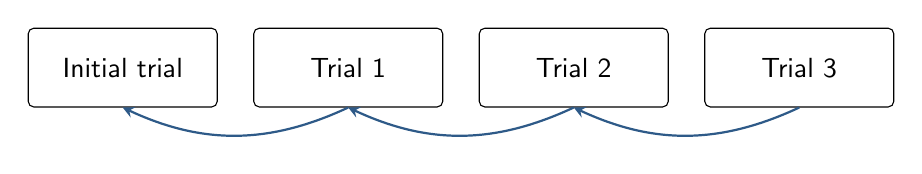
\begin{tikzpicture}[
        trial/.style={
            draw,
            rounded corners=2pt,
            minimum width=2.4cm,
            minimum height=1.0cm,
            align=center
        },
        ref/.style={
            ->,
            >=stealth,
            thick,
            accent
        },
        node distance=0.45cm
    ]

    \node[trial] (t1) {Initial trial};
    \node[trial, right=of t1] (t2) {Trial 1};
    \node[trial, right=of t2] (t3) {Trial 2};
    \node[trial, right=of t3] (t4) {Trial 3};

    % Each decision trial refers to the immediately previous trial
    \draw[ref] (t2.south) to[bend left=25] (t1.south);
    \draw[ref] (t3.south) to[bend left=25] (t2.south);
    \draw[ref] (t4.south) to[bend left=25] (t3.south);

    \end{tikzpicture}

    \caption{
        Reference structure in a ``Previous'' block.
        Each decision trial is compared with the immediately previous trial.
    }
    \label{fig:previous-reference}
\end{figure}


\section{"First" Block}


\begin{figure}[H]
    \centering

    \includegraphics[
        width=0.48\textwidth
    ]{\FirstInitialImage}

    \caption{Example of an initial trial in a ``First'' block.}
    \label{fig:first-initial}
\end{figure}


\begin{figure}[H]
    \centering

    \begin{subfigure}[t]{0.48\textwidth}
        \centering
        \includegraphics[width=\linewidth]{\FirstSameImage}
        \caption{Same rule}
        \label{fig:first-same}
    \end{subfigure}
    \hfill
    \begin{subfigure}[t]{0.48\textwidth}
        \centering
        \includegraphics[width=\linewidth]{\FirstDifferentImage}
        \caption{Different rule}
        \label{fig:first-different}
    \end{subfigure}

    \caption{
        Example decision trials in a ``First'' block.
        The current rule is always compared with the rule from the initial trial,
        regardless of whether the current rule is the same or different.
    }
    \label{fig:first-decisions}
\end{figure}

\vspace{0.5cm}

\begin{figure}[H]
    \centering

    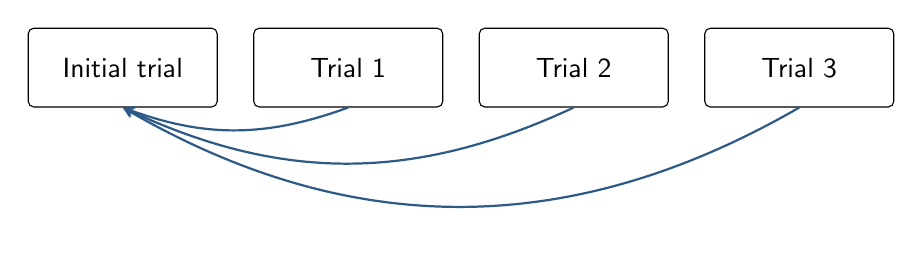
\begin{tikzpicture}[
        trial/.style={
            draw,
            rounded corners=2pt,
            minimum width=2.4cm,
            minimum height=1.0cm,
            align=center
        },
        ref/.style={
            ->,
            >=stealth,
            thick,
            accent
        },
        node distance=0.45cm
    ]

    \node[trial] (t1) {Initial trial};
    \node[trial, right=of t1] (t2) {Trial 1};
    \node[trial, right=of t2] (t3) {Trial 2};
    \node[trial, right=of t3] (t4) {Trial 3};

    % Every decision trial refers to the initial trial
    \draw[ref] (t2.south) to[bend left=20] (t1.south);
    \draw[ref] (t3.south) to[bend left=25] (t1.south);
    \draw[ref] (t4.south) to[bend left=30] (t1.south);

    \end{tikzpicture}

    \caption{
        Reference structure in a ``First'' block.
        Every decision trial is compared with the initial trial.
    }
    \label{fig:first-reference}
\end{figure}

\end{document}
